\section{Atmosph�re: Begriffe}
\subsection{Kapitel 3: Strahlung}
\begin{tabular}{p{4cm} p{15cm}}
Schwarzer K�rper (sK)	& \begin{itemize}
				\item Ein sK absorbiert elektromagnetische Strahlung vollst�ndig. Somit (wegen Kirchhoffschem Strahlungsgesetz) ist sein (W�rme-) Emissionsverm�gen im Vergleich zu beliebigen K�rper maximal ($\epsilon = 1$)
				\item Ein sK l�sst keine Strahlung hindurch und spiegelt oder streut nichts.
				\item Ein beliebiger K�rper kann bei keiner Wellenl�nge mehr Strahlung aussenden als ein sK
                	  \end{itemize}\\
Wiensches Verschiebungsgesetz	& \begin{tabular}[t]{l}
                             	   $\boxed{\lambda_{max} \cdot T = 2.898\cdot 10^{-3}$ m K$}$\\
				   $[\lambda_{max}] = \mu$ m; Wellenl�nge bei der die gr�sste Strahlungsintensit�t auftritt.\\
				   $[T] =$ K; absolute Temperatur der strahlenden Fl�che\\
				   $\lambda_{max} = \frac{d}{d\lambda} J(\lambda)$\\
				   $\lambda_{max, Sonne} \approx 500$ nm\\
				   $\lambda_{max, Erde} \approx 10^4$ nm
				  \end{tabular}\\
Planck'sches Strahlungsgesetz	& \begin{tabular}[t]{l}
                             	   $\boxed{J(\lambda)d\lambda = \frac{2\pi hc^2}{\lambda^5}\frac{1}{e^{hc/\lambda k_B T}-1} d\lambda dA}$\\
				   Strahlungsenergie pro Wellenl�ngenintervall pro Fl�cheneinheit\\
                             	  \end{tabular}\\
Stefan-Boltzmann-Gesetz	& \begin{tabular}[t]{l}
                        	   $\boxed{P = \sigma A \epsilon T^4}$\\
				   $[P] =$ W; Strahlungsenergie, die auf eine Seite von der Fl�che $A$ abgestrahlt wird.\\
				   $\sigma = 5.67\cdot 10^{-8} \tfrac{W}{m^2K^4}$, Stefan-Boltzmann-Konstante\\
				   $\epsilon \leq 1:$ Emissionsverm�gen\\
				   $P = \int_{\lambda = 0}^{\infty} \int_{Halbraum} J(\lambda) dA d\lambda$
			  \end{tabular}\\
Absorption		& Zusammenstoss eines Photons mit einem Partikel, wobei das Photon unterschiedlich stark absorbiert werden kann. Absorbiert Partikel X ein Photon, so hat es mehr Energie, d.h. es\\
Albedo			& Prozentualer Anteil der einfallenden Strahlung, der nicht absorbiert wird. Reflexion oder Streuung bspw. durch Aerosole oder Wolken, Erdboden.\\
Treibhausgase		& 1. H$_2$O, 2. CO$_2$, 3. CH$_4$, 4. O$_3$, 5. FCKW, 6. N$_2$O\\
			& Infrarotabsorption (8000 - 20000 nm): v.a. H$_2$O, CO$_2$\\
			& Infrarotfenster (8000 - 12000 nm): fast keine nat�rliche Absorption\\
			& Die oben genannten Gase absorbieren vor allem im IR-Fenster. Dies ist die Definition f�r Treibhausgase.
\end{tabular}
\begin{tabular}{p{4cm} p{15cm}}
Absorptionslinien	& 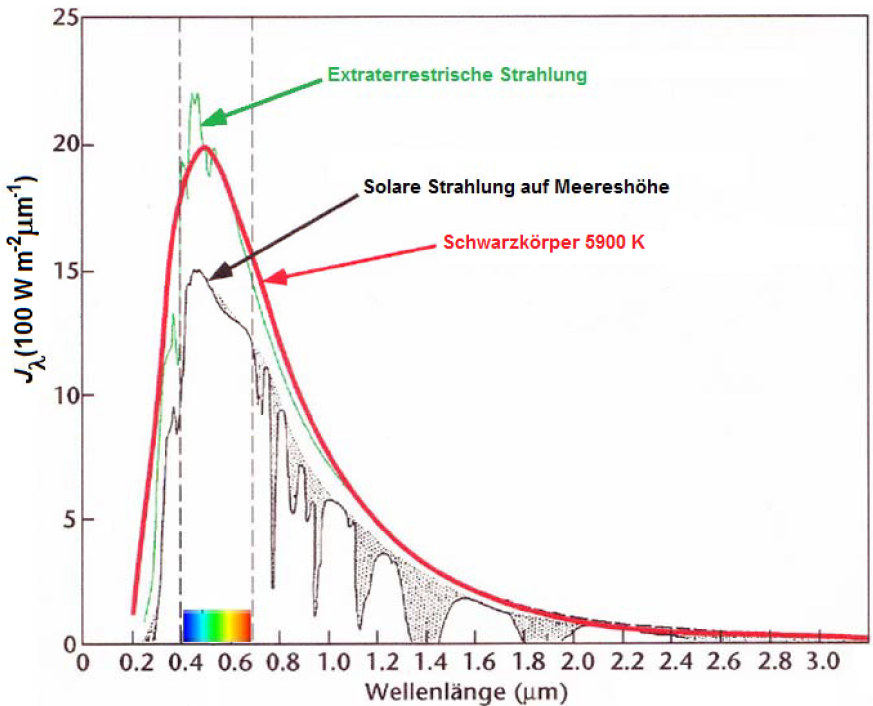
\includegraphics[width = 15cm]{atm_absorptionslinien.png}\\
Wellenl�ngen		& \begin{tabular}[t]{lll}
			    Elektronen�bergang	& UV, sichtbar\\
			    Vibrationen		& kurzwelliges IR\\
			    Rotationen		& langwelliges IR
			  \end{tabular}\\
Strahlungsemission der Erde	& 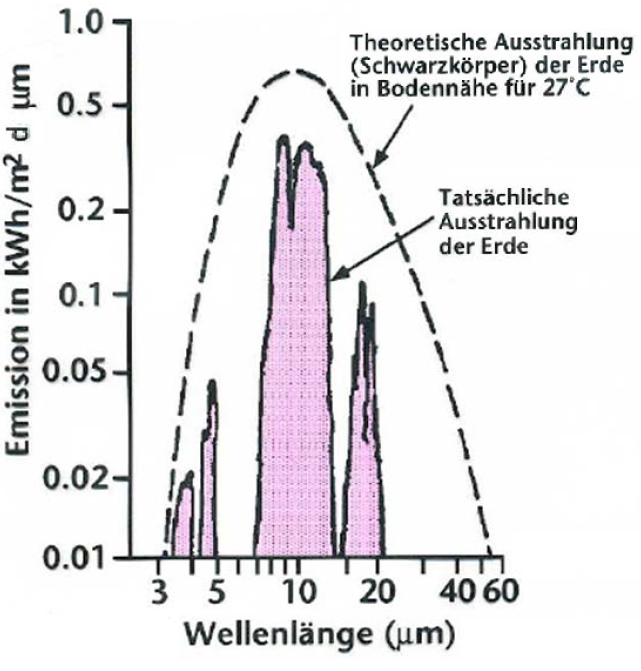
\includegraphics[width = 10cm]{atm_erdemission.png}\\
			& Absorption durch Treibhausgase (Treibhauseffekt). Treibhausgase, die um 10000 nm (IR-Fenster) aktiv sind, haben einen besonders starken Erw�rmungseffekt.
\end{tabular}
\begin{tabular}{p{4cm} p{15cm}}
Strahlungsbudget	& 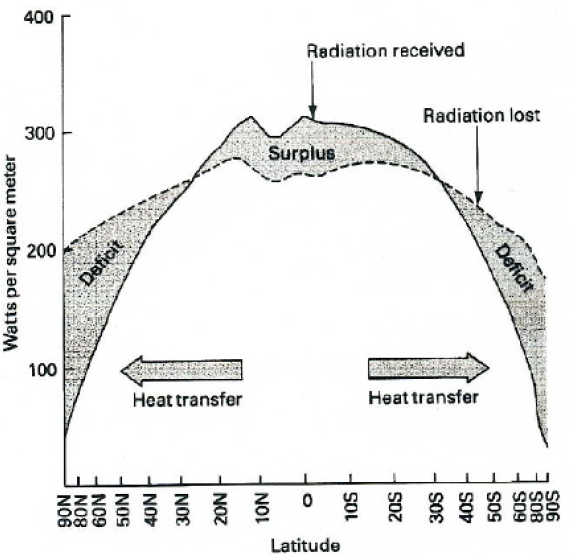
\includegraphics[width = 10cm]{atm_strahlungsbudget.png}\\
			& Sonneneinstrahlung nimmt gegen Pole ab. Albedo nimmt gegen Pole zu. $\Rightarrow$ Am Boden absorbierte Energie nimmt gegen Pole ab. Zum Ausgleich findet ein W�rmetransport statt, mittels Ozean- und Luftstr�mungen (latente W�rme und f�hlbare W�rme)
\end{tabular}

